\subsection{Acetone}

Analoga trattazione \`e stata effettuata nel caso della molecola di acetone.
La geometria iniziale, fornita attraverso z-matrix, possiede configurazione C$_{2v}$,
con gli atomi di idrogeno metilici sul piano, non affacciati.

\begin{figure}[ht]
\begin{center}
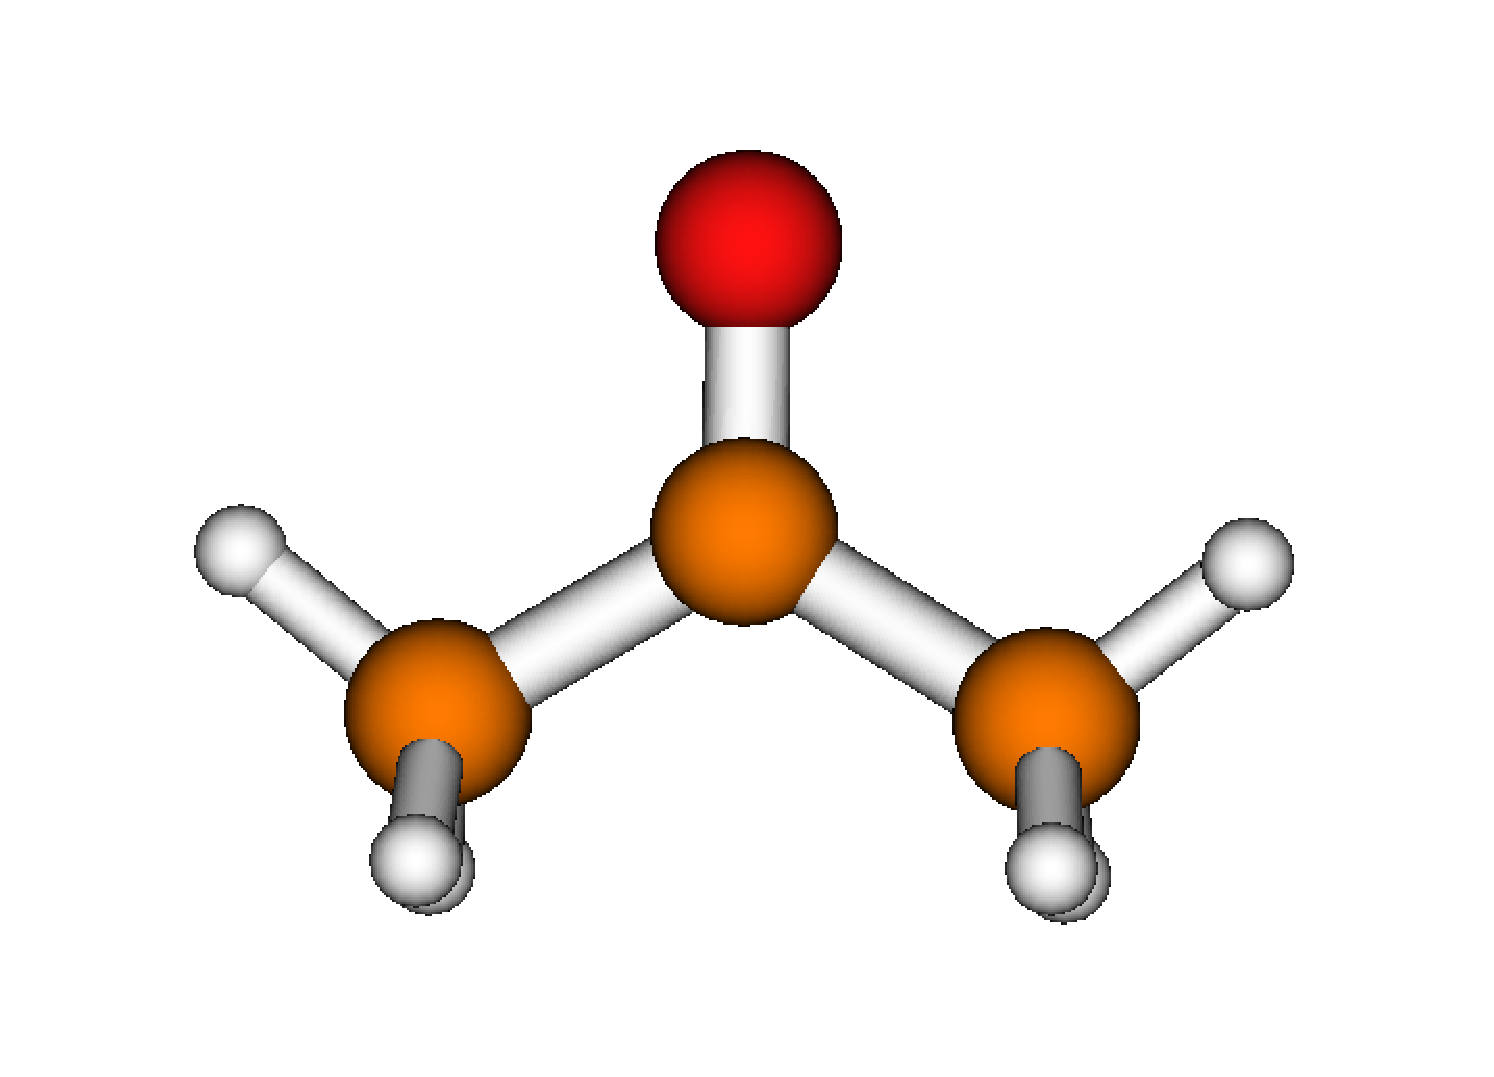
\includegraphics[angle=270,width=7cm,keepaspectratio]{immagini/acetone/geom.eps}
\parbox[h]{12cm}{
\caption{\small Acetone - configurazione spaziale per lo stato fondamentale}
\label{fig:acetone_geom}
}
\end{center}
\end{figure}

L'ottimizzazione di geometria \`e stata effettuata con base 6-311G* a livello CAS,
con uno spazio analogo a quello della formaldeide. La tabella \ref{tab:acetone_geom}
mette a confronto alcuni risultati con il dato sperimentale.
\begin{center}
\begin{threeparttable}
\caption{Acetone - geometria stato fondamentale}
\label{tab:acetone_geom}
\small
\begin{tabular}{|ccc|c|}
\hline
							& CASSCF	& Exp.\tnote{1} \\ 
\hline
$r$(C-O)\tnote{2}			& 1.221		& 1.222				\\
$r$(C-C)\tnote{2}			& 1.511		& 1.507				 \\
$r$(C-H$_1$)\tnote{3}			& 1.081		&			 		 \\
$r$(C-H$_2$)\tnote{3}			& 1.086		&				 	 \\
$\angle$(O-C-C)				& 121.33	& 121.49			 \\
$\angle$(C-C-C)				& 117.33	& 117.02			 \\
\hline
\end{tabular}
\begin{tablenotes}
\parbox[h]{6cm}{
\small
 \item[1] Cfr. \cite{jms-550-551-2000-281}, \cite{jms-120-1986-118} e
 \cite{mp-31-1976-1377}
 \item[] Distanze in Angstroms, angoli in gradi. H$_1$ fa riferimento agli
         idrogeni coplanari al carbonile. H$_2$ agli idrogeni sopra e sotto tale
         piano
}
\end{tablenotes}
\end{threeparttable}
\end{center}
Come si pu\`o notare, la distanza C=O aumenta leggermente, se confrontata
con quella della formaldeide di 1.216 \AA. Ci\`o \`e interpretabile in seguito
all'aumento di interazione sterica tra la nuvola di carica del carbonile e i
gruppi metilici.

La trattazione MCSCF ha richiesto
18 configurazioni, per uno spazio di 6 elettroni in 5 orbitali, illustrati
in figura \ref{fig:acetone_orbitali}. Dal momento che l'acetone possiede la
medesima simmetria della formaldeide, le rappresentazioni irriducibili a cui
apparterranno gli orbitali saranno le medesime elencate in precedenza: A$_1$, B$_1$,
B$_2$ e A$_2$. La distribuzione HF per la molecola di acetone sar\`a quindi
\begin{itemize}
\item 8 di simmetria A$_1$
\item 2 di simmetria B$_1$
\item 5 di simmetria B$_2$
\item 1 di simmetria A$_2$
\end{itemize}

Data la scelta dello spazio CAS, lo spazio inattivo risulta essere
costituito da 7 orbitali di simmetria A$_1$, 1 orbitale di simmetria B$_1$,
4 orbitali di simmetria B$_2$ e 1 orbitale di simmetria A$_2$. Analogamente
al caso della formaldeide, lo stato elettronico finale della transizione
$n_y \rightarrow \pistar$ sar\`a B$_2 \otimes $B$_1 = $A$_2 $.

\begin{figure}[htb]
\begin{center}
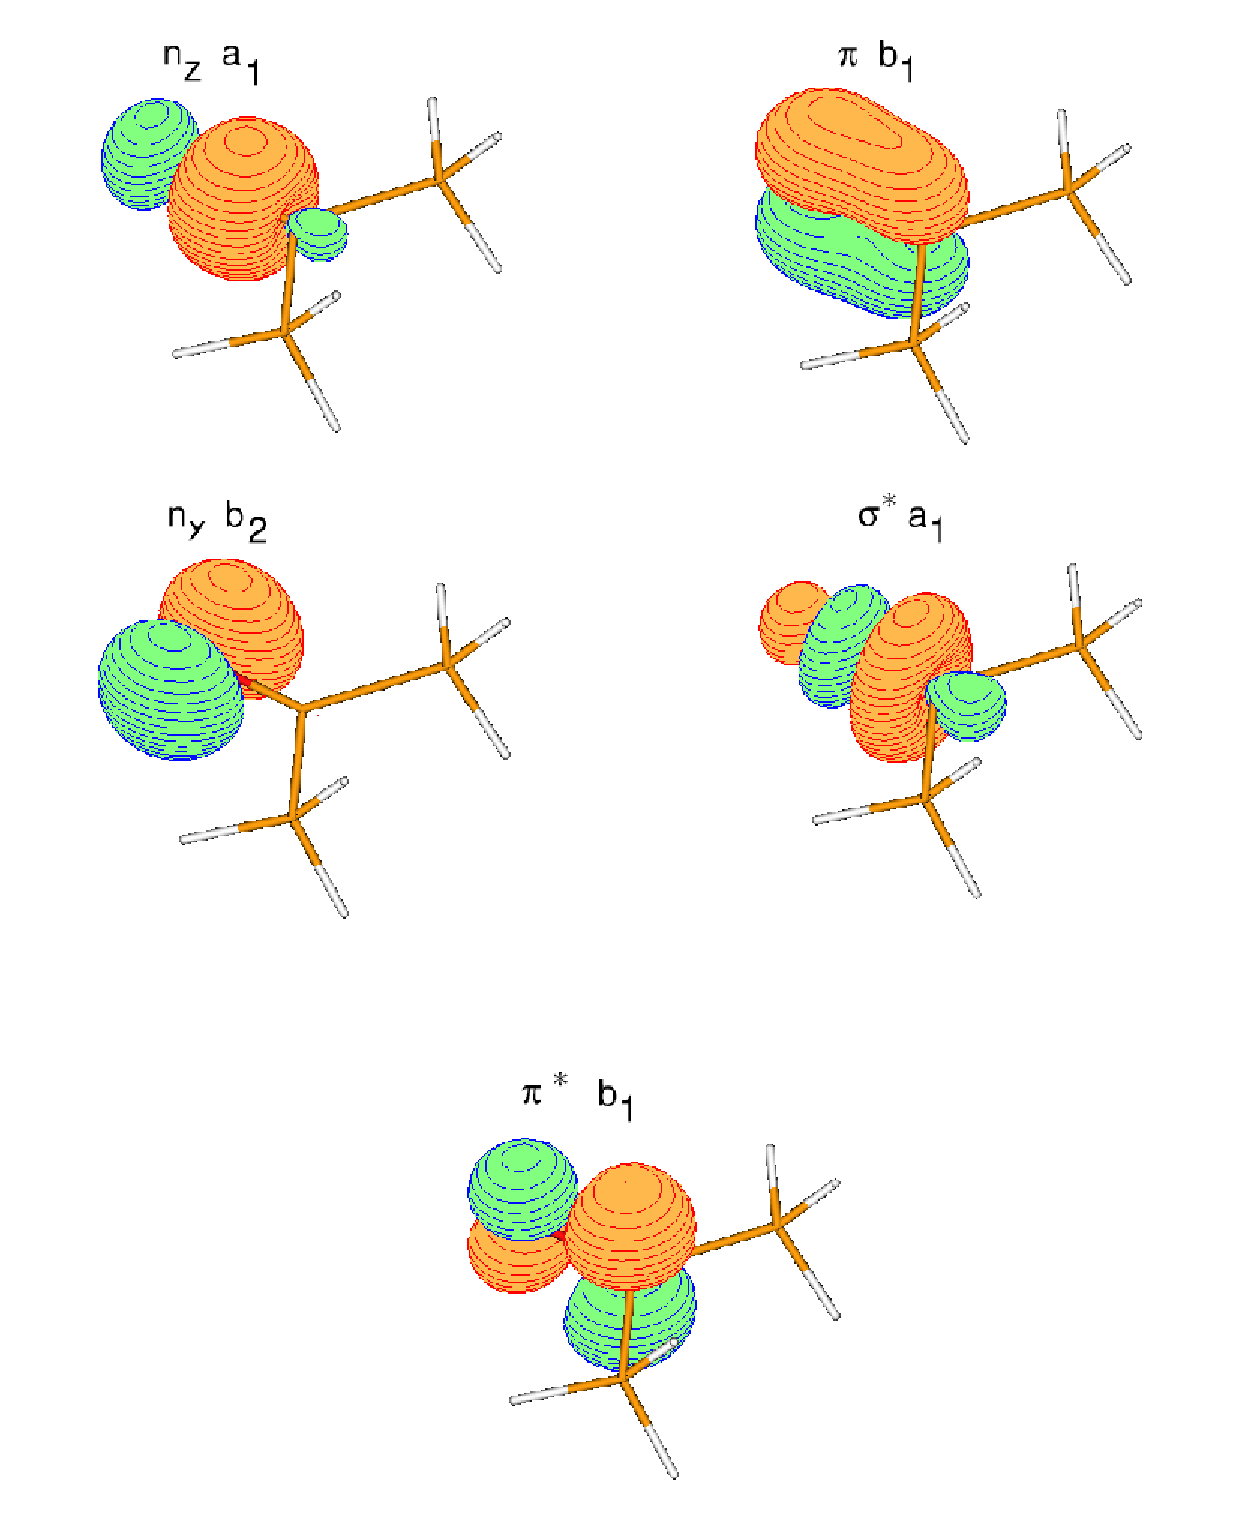
\includegraphics[width=8cm,keepaspectratio]{immagini/acetone/orbitali.eps}
\end{center}
\caption{Spazio CAS per l'acetone}
\label{fig:acetone_orbitali}
\end{figure}

La tabella mostra i numeri di occupazione per lo
stato fondamentale
\begin{verbatim}
 Simmetria A1 : 1.978732113   0.021697330
 Simmetria B1 : 1.938253072   0.062093260 
 Simmetria B2 : 1.999224225
\end{verbatim}

L'energia CASSCF finale per questa base (6-311G*) \`e -192.074240 Hartree.

L'analisi della transizione verticale ha fornito, per lo stato eccitato, un'energia 
-191.895199 Hartree, con una transizione rispetto allo stato fondamentale
di 4.87 eV, contro un valore sperimentale di 4.43 eV (Cfr. \cite{cpl-241-0-1995-26}).
La tabella seguente mostra i numeri di occupazione per lo
stato eccitato
\begin{verbatim}
 Simmetria A1 : 1.984561941   0.015780241 
 Simmetria B1 : 1.996558895   1.003098923
 Simmetria B2 : 1.000000000
\end{verbatim}

Il calcolo effettuato per la transizione adiabatica ha fornito un'energia finale di
-191.932347 Hartree, pari ad una transizione di 3.86 eV contro un valore sperimentale di 3.77 eV
(Cfr. \cite{jcp-111-1-1999-205}). Anche in questo caso, come \`e prevedibile,
il legame carbonilico si allunga in seguito all'occupazione dell'orbitale di
antilegame.
\begin{center}
\begin{threeparttable}
\caption{\small Acetone - geometria di transizione adiabatica}
\label{tab:acetone_geometrie_adiab}
\small
\begin{tabular}{|c|cc|}
\hline
				& CASSCF	& $n_y \rightarrow \pistar$  \\
\hline
$r$(C-O)			& 1.221		& 1.397				\\
$r$(C-C)		& 1.511		& 1.499				 \\
$r$(C-H$_1$)		& 1.080		& 1.084		 		 \\
$r$(C-H$_2$)		& 1.086		& 1.083			 	 \\
$r$(C-H$_3$)		& 1.086		& 1.089			 	 \\
$\angle$(O-C-C)		& 121.33	& 112.13			 \\
$\angle$(C-C-C)		& 117.33	& 121.32			 \\
\hline
\end{tabular}
\begin{tablenotes}
\small
 \item[] Distanze in Angstroms, angoli in gradi
\end{tablenotes}
\end{threeparttable}
\end{center}

\subsubsection{Dipendenza dalla base atomica}

Similmente alla molecola di formaldeide, abbiamo condotto calcoli a
livello CASSCF e perturbativo con le basi
\begin{itemize}
 \item 6-31G
 \item cc-pVDZ
 \item ano-1 (con riduzione 3s2p1d per il carbonio e 2s1p per l'idrogeno)
 \item 6-311G* 
 \item cc-pVTZ
 \item cc-pVQZ
\end{itemize}
i risultati sono mostrati in tabella \ref{tab:acetone_vertical_basis}
\begin{center}
\begin{threeparttable}
\caption{\small Acetone - Energia di transizione $n_y \rightarrow \pistar$ verticale di singoletto, metodi CASSCF e CASSCF/NEV-PT}
\label{tab:acetone_vertical_basis}
{
\small
\begin{tabular}{|c|ccc|ccc|}
\hline
 Base	& \multicolumn{3}{c|}{GS\tnote{1}}				& \multicolumn{3}{c|}{$n_y \rightarrow \pistar$ vert.\tnote{2}} \\
		& CASSCF		& NEV-PT	& NEV-PT	& CASSCF		& NEV-PT & NEV-PT \\
		& 				& SC		& PC		&				& SC 	&	 PC \\
\hline
6-31G	& 0.953869		& 1.263394		& 1.265603		& 4.31			& 4.19		& 4.19		    \\
cc-pVDZ	& 1.048077		& 1.567089		& 1.569608		& 4.84			& 4.50		& 4.50			\\
ano-1	& 1.095777		& 1.612795		& 1.615686 		& 4.87			& 4.54 		& 4.53			\\
6-311G*	& 1.074240		& 1.658429		& 1.660956		& 4.87 			& 4.53		& 4.54 			\\
cc-pVTZ & 1.104413		& 1.810794		& 1.813551		& 4.90			& 4.51 		& 4.51			\\
\hline
\hline
Exp.\tnote{3}	&				& 				&				& \multicolumn{3}{c|}{4.43} \\
\hline
\end{tabular}
}
\begin{tablenotes}
\small
 \item[1] Energia come -(191 + valore) Hartree.
 \item[2] Valori in eV.
 \item[3] Cfr. \cite{cpl-241-0-1995-26}
\end{tablenotes}
\end{threeparttable}
\end{center}

Per quanto riguarda la transizione adiabatica, in tabella \ref{tab:acetone_adiab_basis},
si \`e nuovamente tenuto conto della differenza di ZPE tra lo stato fondamentale e quello eccitato.

\begin{center}
\begin{threeparttable}
\caption{\small Acetone - Energia di transizione $n_y \rightarrow \pistar$ adiabatica di singoletto, metodi CASSCF e CASSCF/NEV-PT}
\label{tab:acetone_adiab_basis}
{
\small
\begin{tabular}{|c|ccc|ccc|}
\hline
Base	& ZPE		& ZPE 			& $\Delta$ZPE	& CASSCF & NEV-PT & NEV-PT \\
		& (GS)		& (Ecc.)		& 				& ZPE 	& SC/ZPE & PC/ZPE \\
\hline
6-31G	& 2.437			& 2.382				& -0.055		&  3.40		 & 3.36 		  & 3.38		\\
cc-pVDZ & 2.402			& 2.350				& -0.052		&  3.81		 & 3.70			  & 3.72		\\
ano-1	& 2.419 		& 2.369				& -0.050		&  3.81 	 & 3.69		  	  & 3.70		\\
6-311G* & 2.414			& 2.367				& -0.047		&  3.81		 & 3.72			  & 3.75		\\
cc-pVTZ & 2.399         & 2.350				& -0.049		&  3.84		 & 3.78		 	  & 3.80		\\
\hline
\hline
Exp.\tnote{1} &				& 					& 				& \multicolumn{3}{c|}{3.77}					\\
\hline
\end{tabular}
}
\begin{tablenotes}
\small
 \item[1] Cfr. \cite{jcp-111-1-1999-205}
 \item[] Valori in eV
\end{tablenotes}
\end{threeparttable}
\end{center}

Nelle figure \ref{fig:acetone_gs}, \ref{fig:acetone_vert} e
\ref{fig:acetone_adiab} sono diagrammate le energie assolute degli stati
fondamentale, eccitato verticale ed eccitato adiabatico rispettivamente,
a livello CASSCF (linea rossa), NEV-PT/SC (linea verde) e NEV-PT/PC
(linea blu).
\begin{figure}[ht]
\begin{center}
\includegraphics[angle=270,width=10cm,keepaspectratio]{immagini/acetone/gs.eps}
\parbox[h]{12cm}{
\caption{\small Acetone - Energia dello stato fondamentale a livello CASSCF (linea rossa),
NEV-PT/SC (linea verde) e NEV-PT/PC (linea blu) come funzione della base
atomica.}
\label{fig:acetone_gs}
}
\end{center}
\end{figure}
\begin{figure}[ht]
\begin{center}
\includegraphics[angle=270,width=10cm,keepaspectratio]{immagini/acetone/vert.eps}
\parbox[h]{12cm}{
\caption{\small Acetone - Energia dello stato eccitato (transizione verticale)
a livello CASSCF (linea rossa), NEV-PT/SC (linea verde) e NEV-PT/PC (linea blu)
come funzione della base atomica. }
\label{fig:acetone_vert}
}
\end{center}
\end{figure}
\begin{figure}[ht]
\begin{center}
\includegraphics[angle=270,width=10cm,keepaspectratio]{immagini/acetone/adiab.eps}
\parbox[h]{12cm}{
\caption{\small Acetone - Energia dello stato eccitato (transizione adiabatica)
a livello CASSCF (linea rossa), NEV-PT/SC (linea verde) e NEV-PT/PC (linea blu)
come funzione della base atomica. }
\label{fig:acetone_adiab}
}
\end{center}
\end{figure}
\pagebreak
\clearpage
Graficando l'energia delle transizioni verticale e adiabatica possiamo notare come
la trattazione perturbativa porti a migliori risultati anche in questo caso.
\begin{figure}[ht]
\begin{center}
\includegraphics[angle=270,width=9cm,keepaspectratio]{immagini/acetone/energie_vert.eps} \\
\includegraphics[angle=270,width=9cm,keepaspectratio]{immagini/acetone/energie_adiab.eps}
\parbox[h]{12cm}{
\caption{\small Acetone - energia di transizione verticale (in alto) e adiabatica (sopra) su basi differenti a livello CASSCF (linea rossa), NEV-PT/SC (linea verde) e NEV-PT/PC (linea blu) come funzione della base atomica.}
\label{fig:acetone_energie_vert_adiab}
}
\end{center}
\end{figure}
\clearpage
%\begin{figure}[ht]
%\begin{center}
%\includegraphics[angle=270,width=6cm,keepaspectratio]{immagini/acetone/energie_adiab.eps}
%\parbox[h]{12cm}{
%\caption{\small Acetone - energia di transizione adiabatica su basi differenti a livello CASSCF (linea rossa), NEV-PT/SC (linea verde) e NEV-PT/PC (linea blu) come funzione della base atomica.}
%\label{fig:acetone_energie_adiab}
%}
%\end{center}
%\end{figure}
%\clearpage
